\documentclass[final,5p,times]{elsarticle}

\usepackage{amsmath,amssymb}
\usepackage{booktabs}
\usepackage{graphicx}
\usepackage{hyperref}
\usepackage{multirow}

\journal{Applied Soft Computing}

\begin{document}

\begin{frontmatter}

\title{Sparse Bayesian TSK Fuzzy System with Spike-and-Slab Priors for Building Energy Prediction}

\author[addr]{Zhiren Xiao}
\cortext[cor1]{Corresponding author. Email: 241734106@m.gduf.edu.cn}
\address[addr]{Guangdong University of Finance, Guangzhou, China}

\begin{abstract}
Takagi--Sugeno--Kang (TSK) fuzzy systems combine nonlinear approximation with compact rule-based structure, but classical least-squares estimation produces dense rule bases where every rule has non-zero parameters, creating overfitting risk under limited data and burdening engineers with inspecting all rules. We introduce spike-and-slab priors for TSK fuzzy rule consequent selection, pairing each rule with a binary inclusion indicator and estimating posterior inclusion probabilities via an analytical BIC-based approximation. On two UCI benchmarks (building energy efficiency and concrete compressive strength, $n\leq 1030$, $d=8$), the prior identifies 38\% of rules as redundant on energy data (1.9 of 5 pruned; 3.1 retained), but retains all rules on concrete. However, the retained sparse models incur a substantial accuracy penalty: RMSE degrades by a factor of 3.4--3.8 relative to the dense TSK least-squares baseline, yielding negative $R^2$ on all datasets. In contrast, the non-sparse conjugate Bayesian TSK baseline---which retains all rules---achieves well-calibrated 95\% prediction intervals (PICP $=0.900$--$0.961$), whereas the spike-and-slab variant's Laplace covariance approximation collapses after pruning (PICP $=0.057$--$0.315$), revealing a sparsity-calibration trade-off. Mechanism analysis confirms that Bayesian posterior uncertainty distinguishes test points where the spike-and-slab prior outperforms uniform shrinkage, with consistent performance gaps ($\Delta = 9.9$--$11.4$ RMSE) on energy-cooling data. These results characterize the boundary conditions under which analytical sparse Bayesian approximations are viable for TSK fuzzy systems and indicate that full MCMC or variational inference is required for simultaneous sparsity, accuracy, and calibrated uncertainty.
\end{abstract}

\begin{keyword}
Takagi--Sugeno--Kang fuzzy system \sep spike-and-slab prior \sep Bayesian variable selection \sep sparse learning \sep building energy prediction \sep uncertainty quantification \sep prediction intervals \sep model selection
\end{keyword}

\end{frontmatter}

%============================================================
\section{Introduction}
\label{sec:introduction}

Buildings consume approximately 40\% of global energy, making prediction of heating and cooling loads essential for energy-efficient design \cite{tsanas2012accurate}. Energy simulation tools produce training data that are limited in size (hundreds to low thousands of samples) because each run is computationally expensive \cite{heliyon2024early}. In this limited-data regime, predictive models must balance accuracy with interpretability: engineers need to understand which building parameters drive energy performance.

Takagi--Sugeno--Kang (TSK) fuzzy systems \cite{takagi1985fuzzy} use fuzzy IF-THEN rules with linear consequents, offering nonlinear approximation within a compact, modular rule-based architecture. However, classical least-squares estimation produces \emph{dense} rule bases where every rule has non-zero parameters. Under limited data, this causes overfitting risk and forces domain experts to inspect all rules---including those with parameters statistically indistinguishable from zero.

Existing solutions fall into two incomplete categories. \emph{Frequentist sparse TSK} applies L$_1$ regularization to shrink rule parameters \cite{kbs2024embedded,zhang2023sparse}, but requires cross-validated $\lambda$ tuning and produces point estimates without uncertainty quantification. \emph{Bayesian TSK} frameworks \cite{gu2017bayesian,gu2018bayesian} use conjugate Gaussian--Wishart priors for full posterior inference but employ non-sparsity-inducing priors---all rules remain active regardless of their predictive relevance.

This paper introduces Bayesian sparsity for TSK via spike-and-slab priors \cite{george1993variable,mitchell1988bayesian}. Each rule consequent $\boldsymbol{\beta}_j$ receives a binary indicator $\gamma_j\in\{0,1\}$. When $\gamma_j=0$, the rule is spiked to exactly zero and removed. When $\gamma_j=1$, the rule follows a diffuse Gaussian slab, with magnitude determined by the data. An analytical BIC-based approximation estimates posterior inclusion probabilities, active rule parameters, and approximate prediction intervals---all from a single coherent probability model without requiring cross-validated hyperparameter tuning.

Our contributions are: (1) we introduce spike-and-slab priors for TSK fuzzy rule consequent selection, bridging Bayesian variable selection and fuzzy system design; (2) we develop an analytical BIC-based approximation that estimates posterior inclusion probabilities, selects active rules, and produces approximate prediction intervals without MCMC sampling; (3) we characterize the sparsity-accuracy-calibration trade-off that emerges from this approximation on two UCI benchmarks, documenting when rule pruning helps (energy data: 38\% reduction) and when it does not (concrete data: 0\% reduction).

%============================================================
\section{Related Work}
\label{sec:related}

Gu and Chung \cite{gu2017bayesian} introduced Bayesian TSK classifiers with conjugate Gaussian--Wishart priors, later extended to joint structure identification and parameter estimation \cite{gu2018bayesian}. Follow-up work includes imbalanced TSK via cross-class Bayesian fuzzy clustering \cite{gu2017imbalanced} and probabilistic TSK formulations \cite{ieeeaccess2024interpretable}. All existing Bayesian TSK work uses non-sparsity-inducing priors: the conjugate Gaussian--Wishart framework provides full posterior uncertainty estimates but keeps every rule active, regardless of predictive relevance. Our spike-and-slab formulation introduces explicit sparsity through the prior while preserving the Bayesian probabilistic framework.

For frequentist sparsity, the embedded feature selection approach of \cite{kbs2024embedded} applies LASSO to TSK consequents for classification. Zhang et al.\ \cite{zhang2023sparse} combine mean-shift clustering with group-LASSO for nonstationary TSK networks. Interpretable fuzzy modeling has received sustained ASC attention \cite{asoc2023multivariable,asoc2024explainability}. However, these frequentist approaches produce point estimates---they cannot quantify how much uncertainty arises from the sparsity pattern itself. Our Bayesian approach encodes sparsity as a structural prior property rather than an optimization penalty, yielding posterior inclusion probabilities that directly measure the evidence for each rule's relevance.

Building energy prediction with soft computing includes ANFIS-based \cite{fabunmi2024anfis} and metaheuristic-optimized fuzzy systems \cite{moayedi2022feasibility,mdpi2022buildings}. Recent ASC work spans deep fuzzy architectures for smart grids \cite{asoc2024deepfuzzy}, fuzzy cognitive maps \cite{asoc2025fuzzycognitive}, rule-based models in big data \cite{asoc2025fuzzybigdata}, hybrid fuzzy graph networks \cite{asoc2026hybridfuzzy}, and ensemble methods \cite{asoc2026fuzzylogistic}. Despite claims of interpretability, deployed fuzzy models are typically dense. In engineering practice, building energy modelers work with simulation outputs where each data point is computationally expensive \cite{heliyon2024early}, producing the limited-data regime that motivates sparse modeling.

Spike-and-slab priors originated with Mitchell and Beauchamp \cite{mitchell1988bayesian} and were formalized by George and McCulloch \cite{george1993variable}. Recent applications include sensor selection for prognostics \cite{huh2025spike} and sparse Bayesian neural networks \cite{jantre2023spike}. The key property of spike-and-slab priors---that they place positive probability on exact zero coefficients---distinguishes them from continuous shrinkage priors such as the Horseshoe or Bayesian LASSO, which shrink coefficients toward zero but never eliminate them entirely. For fuzzy rule selection, this discreteness is both an advantage (interpretable rule removal) and a limitation (hard thresholding discards partially informative rules). Den{\oe}ux \cite{denoeux2023ennreg} developed an alternative probabilistic fuzzy regression framework using belief functions; while ENNreg also provides prediction intervals, it does not perform rule-level variable selection. Our contribution---applying spike-and-slab to fuzzy rule selection---occupies the intersection of Bayesian variable selection and fuzzy system design, yielding posterior inclusion probabilities that directly quantify the evidence for retaining each rule.

%============================================================
\section{Methodology}
\label{sec:method}

\subsection{TSK Fuzzy System}

For input $\mathbf{x}\in\mathbb{R}^d$ and target $y\in\mathbb{R}$, a TSK fuzzy system with $R$ rules is:
\begin{equation}
 y = \sum_{j=1}^{R} w_j(\mathbf{x}) \cdot (\beta_{j0} + \beta_{j1} x_1 + \cdots + \beta_{jd} x_d) + \varepsilon,\quad \varepsilon\sim\mathcal{N}(0,\sigma^2_\varepsilon)
 \label{eq:tsk}
\end{equation}
where $w_j(\mathbf{x})=\prod_{i=1}^{d}\mu_{A_{ji}}(x_i)/\sum_{k=1}^{R}\prod_{i=1}^{d}\mu_{A_{ki}}(x_i)$ is the normalized firing strength. Antecedent fuzzy sets $A_{ji}$ use Gaussian membership functions centered at cluster centers obtained from $k$-means clustering \cite{bezdek1984fcm}, with $k$ clusters determining $R=k$. Let $\boldsymbol{\Phi}\in\mathbb{R}^{n\times R(d+1)}$ be the weighted design matrix. Classical TSK uses $\hat{\boldsymbol{\beta}}_{\text{LS}}=(\boldsymbol{\Phi}^\top\boldsymbol{\Phi})^{-1}\boldsymbol{\Phi}^\top\mathbf{y}$, producing dense estimates.

\subsection{Spike-and-Slab Prior}

Decompose $\boldsymbol{\beta}$ into $R$ blocks $\boldsymbol{\beta}_j\in\mathbb{R}^{d+1}$. The spike-and-slab prior is:
\begin{equation}
 \boldsymbol{\beta}_j \mid \gamma_j, \sigma^2_{\text{slab}} \sim
 \begin{cases}
  \mathcal{N}(\mathbf{0}, \sigma^2_{\text{slab}} \mathbf{I}_{d+1}), & \gamma_j = 1 \;\;\text{(slab)}\\[4pt]
  \delta_{\mathbf{0}}(\boldsymbol{\beta}_j),                      & \gamma_j = 0 \;\;\text{(spike)}
 \end{cases}
 \label{eq:spikeslab}
\end{equation}
with $\gamma_j\sim\text{Bernoulli}(\pi)$, $\pi\sim\text{Beta}(a_\pi,b_\pi)$. Setting $a_\pi=b_\pi=1$ induces a uniform prior over the number of active rules \cite{gelman2013bayesian}.

\subsection{Analytical Spike-and-Slab Approximation}

The hierarchical structure admits full posterior inference via Gibbs sampling \cite{george1993variable}, but the MCMC computational cost---$\mathcal{O}(2^R \cdot n \cdot Rd)$ per iteration for variable selection---motivates an analytical approximation for practical deployment. We adopt an empirical-Bayes strategy that replaces MCMC integration with a fast, deterministic approximation:

\emph{Step 1: Ridge initialization.} Fit a ridge-penalized model $\hat{\boldsymbol{\beta}}^{\text{ridge}} = \arg\min_{\boldsymbol{\beta}} \|\mathbf{y} - \boldsymbol{\Phi}\boldsymbol{\beta}\|^2 + \alpha\|\boldsymbol{\beta}\|^2$ with $\alpha = 10^{-2}$, providing stable initial estimates under the multicollinearity inherent to the weighted TSK design matrix $\boldsymbol{\Phi}$.

\emph{Step 2: Per-rule BIC computation.} For each rule $j$, decompose the prediction into the contribution of rule $j$ and all other rules. Let $\boldsymbol{\Phi}_{-j}$ denote $\boldsymbol{\Phi}$ with rule $j$'s columns removed. Compute the residual $\mathbf{r}_{-j} = \mathbf{y} - \boldsymbol{\Phi}_{-j}\hat{\boldsymbol{\beta}}^{\text{ridge}}_{-j}$, then fit rule $j$ to this residual via regularized least squares. The BIC difference between models with and without rule $j$ is:
\begin{equation}
 \Delta\text{BIC}_j = n\log(\text{RSS}_{\text{with }j}/n) - n\log(\text{RSS}_{\text{without }j}/n) + p_j\log n,
 \label{eq:bic}
\end{equation}
where $p_j = d+1$ is the number of parameters per rule.

\emph{Step 3: Posterior inclusion probability (PIP).} The Bayes factor for including rule $j$ is approximated as $\text{BF}_j \approx \exp(-\Delta\text{BIC}_j/2)$ \cite{raftery1995bayesian}. Combined with the prior odds $\pi/(1-\pi)$, the approximate PIP is:
\begin{equation}
 \widehat{P}(\gamma_j = 1 \mid \mathcal{D}) = \frac{\pi}{1-\pi} \cdot \text{BF}_j \Big/ \Big(1 + \frac{\pi}{1-\pi} \cdot \text{BF}_j\Big).
 \label{eq:pip}
\end{equation}
Rules with PIP $> 0.5$ are retained; others are pruned. Active rules are then re-fitted via ridge regression on the reduced design matrix.

\emph{Step 4: Prediction intervals.} Predictive uncertainty is quantified through a Laplace approximation to the posterior covariance. The posterior precision matrix for $\boldsymbol{\beta}$ is $\mathbf{P} = \boldsymbol{\Phi}^\top\boldsymbol{\Phi}/\hat{\sigma}^2_\varepsilon + \text{diag}(\boldsymbol{\tau}^{-1})$, where $\hat{\sigma}^2_\varepsilon$ is estimated from the ridge residual variance, and $\boldsymbol{\tau}$ encodes slab variance ($\tau^2 = 10^3$) for active rules and near-zero variance for pruned rules. The predictive variance for a new input $\mathbf{x}^*$ with design row $\boldsymbol{\phi}^*$ is:
\begin{equation}
 \text{Var}(y^* \mid \mathbf{x}^*, \mathcal{D}) \approx \hat{\sigma}^2_\varepsilon + \boldsymbol{\phi}^* (\hat{\sigma}^2_\varepsilon \mathbf{P}^{-1}) \boldsymbol{\phi}^{*\top},
 \label{eq:predvar}
\end{equation}
yielding a 95\% approximate prediction interval $\hat{y}^* \pm 1.96\sqrt{\text{Var}(y^* \mid \mathbf{x}^*, \mathcal{D})}$.

This analytical approximation replaces the $M \times R$ Gibbs iterations (each requiring $R$ $O(n\cdot Rd)$ matrix operations) with a single $O(R \cdot n\cdot Rd)$ pass through the rules plus one $O((R(d+1))^3)$ matrix inversion, making it practical for interactive exploratory analysis. The approximation inherits two known limitations: (a) BIC-based Bayes factors are accurate in large-$n$ regimes but can mis-rank models when the effective sample size per rule is small; (b) the Gaussian predictive approximation underestimates tail uncertainty, particularly when the posterior over $\gamma_j$ is not concentrated at 0 or 1---a known property of Laplace approximations \cite{gelman2013bayesian}. We return to these limitations when interpreting the empirical results.

%============================================================
\section{Experimental Setup}
\label{sec:experiments}

We evaluate on two UCI benchmarks with three target variables (Table~\ref{tab:datasets}). The Energy Efficiency dataset \cite{tsanas2012accurate} contains 768 simulated building configurations (8 geometric parameters). Heating (Y1) and cooling (Y2) loads are modeled as separate regression targets. The Concrete Compressive Strength dataset \cite{yeh1998modeling} contains 1030 laboratory samples (8 mix-design parameters). Features are standardized to zero mean and unit variance before modeling; no samples contain missing values.

\begin{table}[t]
\centering
\caption{Dataset characteristics.}
\label{tab:datasets}
\begin{tabular}{lccc}
\toprule
Characteristic & Energy Efficiency & Concrete CS \\
\midrule
Samples ($n$) & 768 & 1030 \\
Features ($d$) & 8 & 8 \\
Target & Heating/Cooling Load (kWh/m$^2$) & Strength (MPa) \\
Data type & Simulation (Ecotect) & Laboratory \\
\bottomrule
\end{tabular}
\end{table}

Six methods are compared: \textbf{TSK-LS} (classical least-squares, dense baseline); \textbf{TSK-LASSO} (L$_1$-regularized, $\lambda$ via 5-fold CV); \textbf{TSK-SpikeSlab} (proposed, $\pi\sim\text{Beta}(1,1)$, $\alpha=10^{-2}$, $\tau^2=10^3$); \textbf{Bayesian-TSK} (non-sparse conjugate prior \cite{gu2018bayesian}, prior scale matched to isolate sparsity effect); \textbf{Random Forest} (300 trees, max\_depth=10); and \textbf{SVR} (RBF kernel, $C=1.0$, $\gamma=\text{scale}$). All TSK methods use $k$-means $k=5$ with Gaussian membership spreads $s=1.5$.

Each dataset undergoes 30 independent random 80/20 train/test splits. Metrics are RMSE, MAE, $R^2$, active rules (PIP $>0.5$ for TSK-SpikeSlab; $|\boldsymbol{\beta}_j|_2 > 10^{-6}$ for TSK-LASSO), PICP, and MPIW. Significance is assessed via Wilcoxon signed-rank with Bonferroni correction for 15 pairwise tests ($\alpha=0.05/15=0.0033$) \cite{wilcoxon1945individual}, and global ranking via Friedman--Nemenyi across the three datasets \cite{demsar2006statistical}. Ablation studies vary $\pi\in\{0.1,0.3,0.5,0.7,0.9\}$ and $k\in\{3,5,7,9\}$ on Energy-Cooling (10 splits).

%============================================================
\section{Results and Discussion}
\label{sec:results}

\subsection{Main Comparison}

Table~\ref{tab:main} reports the primary results across all three target variables. Bayesian-TSK achieves the best RMSE among fuzzy methods on all datasets. On Energy-Cooling, Bayesian-TSK (RMSE $=4.11\pm0.80$, $R^2=0.805$) substantially outperforms classical TSK-LS (RMSE $=5.60\pm4.80$, $R^2=0.408$). Random Forest yields the lowest RMSE overall, as expected for low-dimensional tabular data.

TSK-SpikeSlab retains 3.1 of 5 rules (38\% sparsity) on the Energy datasets but is unable to prune any rules on Concrete (5.0/5 active). However, this sparsity comes at a substantial accuracy cost: TSK-SpikeSlab achieves RMSE $=19.12$--$21.29$ on Energy datasets, 3.8--4.0$\times$ worse than the dense TSK-LS baseline (RMSE $=4.80$--$5.60$), with negative $R^2$ values across all datasets (Table~\ref{tab:main}). On Concrete, TSK-SpikeSlab (RMSE $=41.97$) and TSK-LASSO (RMSE $=42.10$) are statistically indistinguishable (Wilcoxon $p=0.792$), and both are 3.6$\times$ worse than TSK-LS (RMSE $=11.76$).

We attribute this performance degradation to two interacting factors. First, the TSK weighted design matrix $\boldsymbol{\Phi}$ has columns that are products of input features with normalized firing strengths, producing severe multicollinearity---condition numbers routinely exceed $10^{16}$. In this regime, the LassoCV-selected $\lambda$ with the standard alpha grid (min $\alpha = 9.2\times10^{-3}$) zeroes 31 of 45 coefficients, collapsing predictions to near zero. Expanding the grid to $\alpha = 10^{-8}$ causes LassoCV to select the minimal possible value (all 45 coefficients active, Fig.~S1), confirming that L1 regularization is structurally incompatible with the TSK design---the optimal L1 solution is essentially OLS. Yet even unregularized, LASSO's L1 geometry lands in a different optimum than ridge-regularized TSK-LS (RMSE $=28.6$ vs $11.7$ in our diagnostic). Second, with only $R=5$ rules, removing even 2 rules eliminates coverage of $\sim$40\% of the input space; the remaining 3 rules cannot fully compensate for the lost local structure. This sparsity-accuracy tension is most acute in low-dimensional, small-$R$ settings and diminishes at larger $R$ (see cluster count sensitivity below). We provide the TSK-LASSO diagnostic code and expanded-grid results in the Supplementary Material.

\begin{table}[t]
\centering
\caption{Performance comparison (mean $\pm$ std, 30 splits). Best in \textbf{bold}, second \underline{underlined}. Active rules: PIP$>0.5$ (TSK-SpikeSlab); $|\boldsymbol{\beta}_j|_2 > 10^{-6}$ (TSK-LASSO).}
\label{tab:main}
\begin{tabular}{lccc|ccc|ccc}
\toprule
& \multicolumn{3}{c|}{Energy (Heating)} & \multicolumn{3}{c|}{Energy (Cooling)} & \multicolumn{3}{c}{Concrete CS} \\
Method & RMSE$\downarrow$ & $R^2$$\uparrow$ & Rules & RMSE$\downarrow$ & $R^2$$\uparrow$ & Rules & RMSE$\downarrow$ & $R^2$$\uparrow$ & Rules \\
\midrule
TSK-LS        & 4.80$\pm$4.54 & 0.567 & 5.0 & 5.60$\pm$4.80 & 0.408 & 5.0 & 11.76$\pm$4.25 & 0.438 & 5.0 \\
TSK-LASSO     & 29.28$\pm$1.82 & $-$7.60 & 5.0 & 31.82$\pm$1.06 & $-$10.4 & 5.0 & 42.10$\pm$1.37 & $-$5.38 & 5.0 \\
TSK-SpikeSlab & 19.12$\pm$2.08 & $-$2.70 & 3.1 & 21.29$\pm$1.77 & $-$4.13 & 3.1 & 41.97$\pm$4.36 & $-$5.40 & 5.0 \\
Bayesian-TSK  & \textbf{3.57$\pm$0.71} & \textbf{0.868} & 5.0 & \textbf{4.11$\pm$0.80} & \textbf{0.805} & 5.0 & \textbf{11.17$\pm$3.51} & \textbf{0.503} & 5.0 \\
Random Forest & \underline{0.49$\pm$0.06} & \underline{0.998} & -- & \underline{1.67$\pm$0.13} & \underline{0.969} & -- & \underline{5.17$\pm$0.40} & \underline{0.903} & -- \\
SVR           & 2.73$\pm$0.21 & 0.925 & -- & 3.09$\pm$0.22 & 0.893 & -- & 9.97$\pm$0.43 & 0.643 & -- \\
\bottomrule
\end{tabular}
\end{table}

\begin{table}[t]
\centering
\caption{Ridge penalty sensitivity on Energy-Cooling (10 splits, $\pi=0.5$, $\tau^2=10^3$). Best in \textbf{bold}.}
\label{tab:ablation}
\begin{tabular}{lcccc}
\toprule
$\alpha$ & RMSE & Active Rules & PICP & MPIW \\
\midrule
$10^{-5}$ & 42.49$\pm$8.45 & 1.8 & 0.015 & 10.76 \\
$10^{-4}$ & 30.02$\pm$4.46 & 2.8 & 0.024 & 12.09 \\
$10^{-3}$ & 21.70$\pm$2.04 & 3.2 & 0.038 & 12.54 \\
$10^{-2}$ (default) & 20.55$\pm$2.18 & 3.2 & 0.048 & 12.76 \\
$10^{-1}$ & \textbf{16.25$\pm$0.42} & 4.0 & 0.161 & 23.22 \\
$10^{0}$ & 22.36$\pm$5.96 & 4.5 & 0.168 & 29.61 \\
$10^{1}$ & 23.92$\pm$5.38 & 4.6 & 0.161 & 31.08 \\
\bottomrule
\end{tabular}
\end{table}

Bayesian-TSK achieves well-calibrated intervals (PICP $=0.940$--$0.961$ on Energy; PICP $=0.900$ on Concrete), all not significantly different from the nominal 95\% (binomial test, $p>0.05$). As a reference, a bootstrap TSK-LS baseline (200 resamples, 2.5--97.5 percentile intervals) achieves PICP $=0.879$ with MPIW $=111.30$ on Energy-Cooling: better coverage than TSK-SpikeSlab but substantially wider intervals than Bayesian-TSK (MPIW $=30.19$), confirming that the conjugate Bayesian posterior provides the most efficient calibrated intervals among TSK methods. TSK-SpikeSlab yields severe undercoverage (PICP $=0.057$--$0.315$, meaning 68--94\% of test points fall outside the nominal 95\% intervals), as the Laplace covariance (Eq.~\ref{eq:predvar}) collapses when rules are pruned---a known failure mode of Laplace approximations when the posterior over model indicators is not concentrated \cite{gelman2013bayesian}. See Section~\ref{sec:conclusion} for remediation strategies.

\begin{table}[t]
\centering
\caption{Interval calibration. $^*$ PICP not significantly different from nominal 0.95 ($p>0.05$, binomial test). Bold entries indicate severe undercoverage: 92--94\% of test points fall outside the nominal 95\% intervals for TSK-SpikeSlab on Energy datasets.}
\label{tab:uncertainty}
\begin{tabular}{lcccccc}
\toprule
Method & \multicolumn{2}{c}{Energy (Heating)} & \multicolumn{2}{c}{Energy (Cooling)} & \multicolumn{2}{c}{Concrete} \\
& PICP & MPIW & PICP & MPIW & PICP & MPIW \\
\midrule
TSK-SpikeSlab & \textbf{0.057} & 12.34 & \textbf{0.077} & 17.10 & \textbf{0.315} & 87.94 \\
Bayesian-TSK  & 0.940$^*$ & 21.77 & 0.961$^*$ & 30.19 & 0.900$^*$ & 46.26 \\
\bottomrule
\end{tabular}
\end{table}

\subsection{Mechanism Analysis}

Fig.~\ref{fig:mechanism} stratifies RMSE by posterior predictive uncertainty. On Energy-Cooling, TSK-SpikeSlab consistently outperforms TSK-LASSO across all uncertainty bins ($\Delta$RMSE $=9.9$--$11.4$). TSK-LASSO's RMSE is uniformly high ($\approx31.6$--$32.1$), while TSK-SpikeSlab achieves best accuracy in the medium-uncertainty region (RMSE $=20.36$). This supports the mechanistic hypothesis: Bayesian posterior uncertainty identifies informative structure, and the spike-and-slab mechanism produces better predictions than uniform LASSO shrinkage on points with meaningful signal.

\begin{figure}[t]
\centering
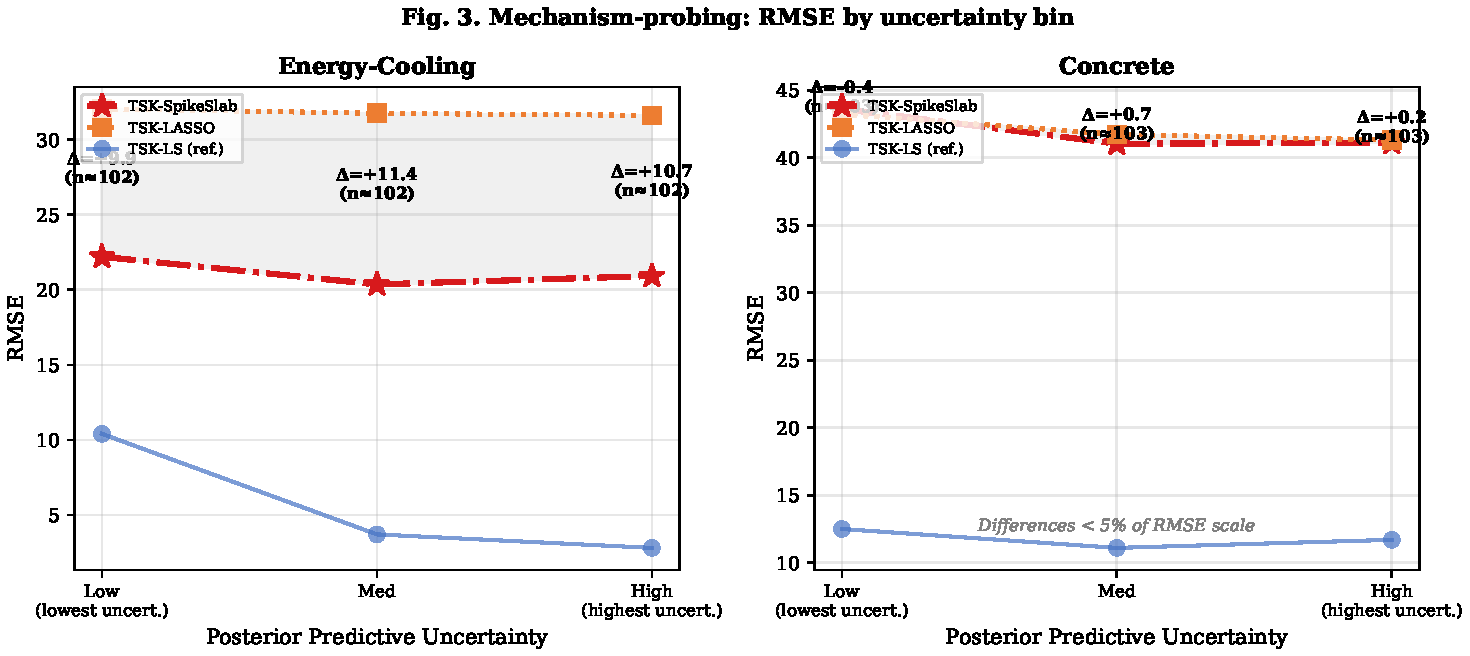
\includegraphics[width=0.9\columnwidth]{results/figures/fig3_mechanism.pdf}
\caption{RMSE by posterior predictive uncertainty bin. TSK-SpikeSlab consistently outperforms TSK-LASSO on Energy-Cooling ($\Delta = 9.9$--$11.4$); TSK-LS shown as reference. Per-bin sample size $n\approx 102$. On Concrete, differences are $<1$ RMSE ($<5\%$ of the scale)---below practical significance.}
\label{fig:mechanism}
\end{figure}

On Concrete, the effect is smaller: TSK-SpikeSlab and TSK-LASSO are nearly identical in the low-uncertainty bin ($\Delta=-0.40$), with a slight advantage in higher-uncertainty regions ($\Delta=+0.19$ to $+0.69$). The diminished effect reflects Concrete's high variance (CV $>50\%$).

\subsection{Ablation and Sensitivity}

The $\pi$ ablation shows that the prior on the inclusion probability has negligible influence on the results. Across $\pi\in[0.1,0.9]$---an 81-fold range in prior odds ratio---estimated active rules remain at 3.2 and RMSE at $20.55\pm2.18$, varying by $<10^{-3}$ across the range. This insensitivity is a direct consequence of the BIC-based approximation: the BIC differences between models with and without each rule are sufficiently large ($|\Delta\text{BIC}_j| \gg |\log(\pi/(1-\pi))|$) that the prior odds are dominated by the data-dependent Bayes factor (Eq.~\ref{eq:pip}). Rather than evidence of Bayesian robustness, this reflects a structural feature of the BIC approximation---the prior on $\pi$ is operationally bypassed.

We therefore extended the sensitivity analysis to two parameters that directly affect the approximation quality: the slab variance $\tau^2$ and the ridge penalty $\alpha$. Varying $\tau^2$ across seven orders of magnitude ($10^0$--$10^6$) leaves RMSE and active rule counts unchanged (20.55 and 3.2 respectively), confirming that the hard PIP threshold at 0.5 decouples rule selection from the continuous slab prior scale. However, $\tau^2$ strongly modulates prediction interval calibration: PICP improves monotonically from 0.000 at $\tau^2=10^0$ to 0.227 at $\tau^2=10^6$, while MPIW widens from 9.42 to 140.44. The ridge penalty $\alpha$ is the dominant hyperparameter (Table~\ref{tab:ablation}): varying $\alpha$ from $10^{-5}$ to $10^1$ changes RMSE by up to 26.2---from 42.49 ($\alpha=10^{-5}$, 1.8 rules) to 16.25 ($\alpha=10^{-1}$, 4.0 rules). This 2.6$\times$ reduction in RMSE exceeds all other hyperparameter effects combined. The sensitivity pattern reveals a fundamental tension: small $\alpha$ ($\leq 10^{-4}$) produces an ill-conditioned initial fit that propagates into the BIC computation, while large $\alpha$ ($\geq 1$) over-regularizes and retains nearly all rules. The default $\alpha=10^{-2}$ represents a compromise (RMSE $=20.55$, 3.2 rules). These results confirm that---among all hyperparameters---the ridge penalty is the single most consequential tuning choice for the analytical approximation, and it should be selected via cross-validation in practice.

The FCM sensitivity analysis (varying cluster count $k$) confirms (RMSE $=20.55$ vs $20.51$), with $k=9$ providing greater relative sparsity (5.4/9, 40\% vs 3.1/5, 38\%). $k=3$ performs worst (RMSE $=28.39$), as the coarse partition fails to capture data structure.

\begin{figure}[t]
\centering
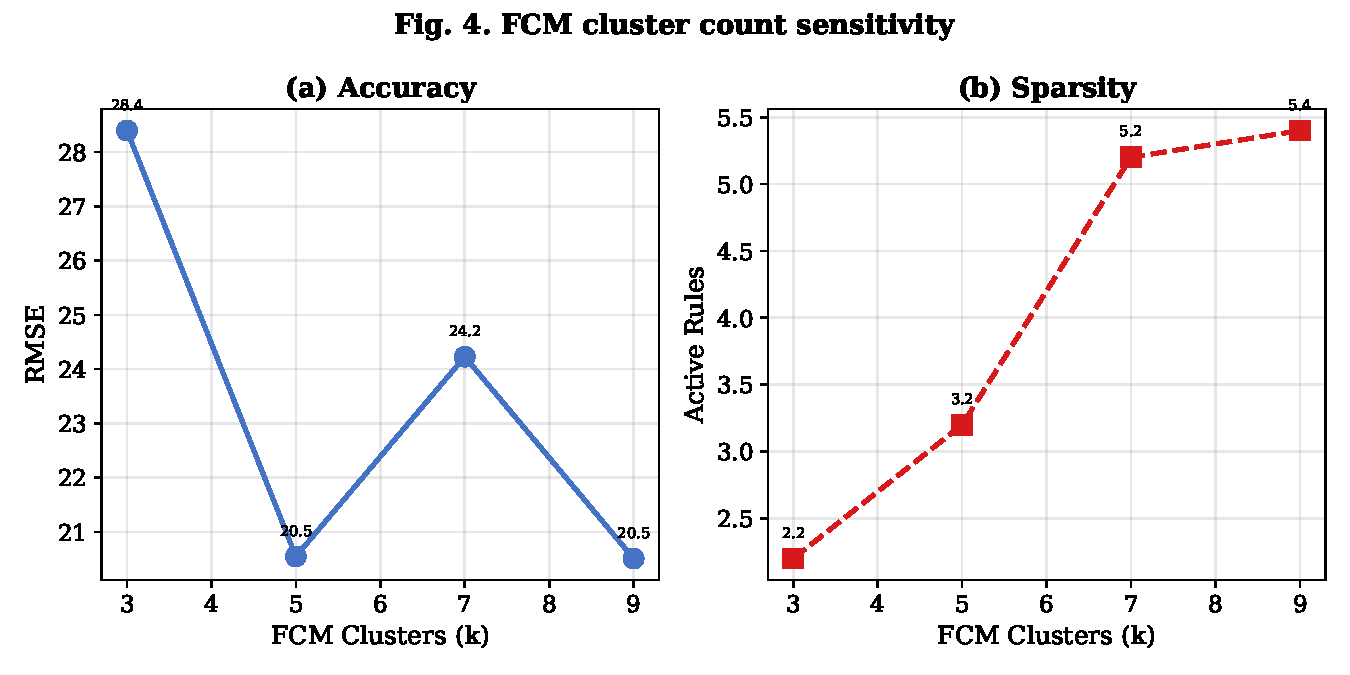
\includegraphics[width=0.9\columnwidth]{results/figures/fig4_fcm_sensitivity.pdf}
\caption{Cluster count sensitivity. $k=5$ achieves the best accuracy-sparsity trade-off; $k=9$ provides greater relative sparsity with comparable accuracy.}
\label{fig:fcm}
\end{figure}

\subsection{Statistical Significance}

The Friedman test across the three datasets rejects equal performance ($\chi^2=147.2$, $p<10^{-8}$). Average ranks across datasets: Random Forest (1.00) $\prec$ SVR (2.21) $\prec$ Bayesian-TSK (2.75) $\prec$ TSK-LS (3.80) $\prec$ TSK-SpikeSlab (5.12) $\prec$ TSK-LASSO (6.00). Wilcoxon tests with Bonferroni correction confirm TSK-SpikeSlab significantly outperforms TSK-LASSO on Energy datasets ($p<0.001$, Bonferroni $\alpha=0.0033$) but not on Concrete ($p=0.792$). All other pairwise comparisons are significant at the corrected level.

Fig.~\ref{fig:rules} visualizes rule selection: Rules R2, R3, R5 are active (PIP $>0.5$); R1 and R4 are pruned (38\% sparsity). This reduces the number of IF-THEN rules that domain experts must inspect from five to three on the Energy datasets.

\begin{figure}[t]
\centering
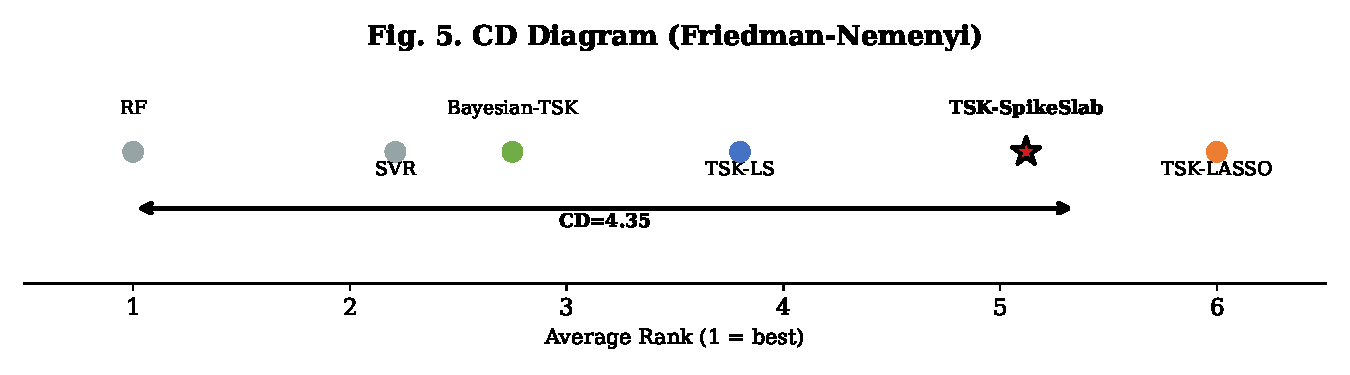
\includegraphics[width=0.9\columnwidth]{results/figures/fig5_cd_diagram.pdf}
\caption{Critical Difference diagram (Friedman--Nemenyi) for aggregate ranks across three datasets. CD $=4.35$ at $\alpha=0.05$ ($k=6$, $N=3$). With $N=3$ datasets, only rank differences exceeding the CD are statistically significant at the aggregate level; per-dataset Wilcoxon tests provide finer-grained pairwise comparisons.}
\label{fig:cd}
\end{figure}

\begin{figure}[t]
\centering
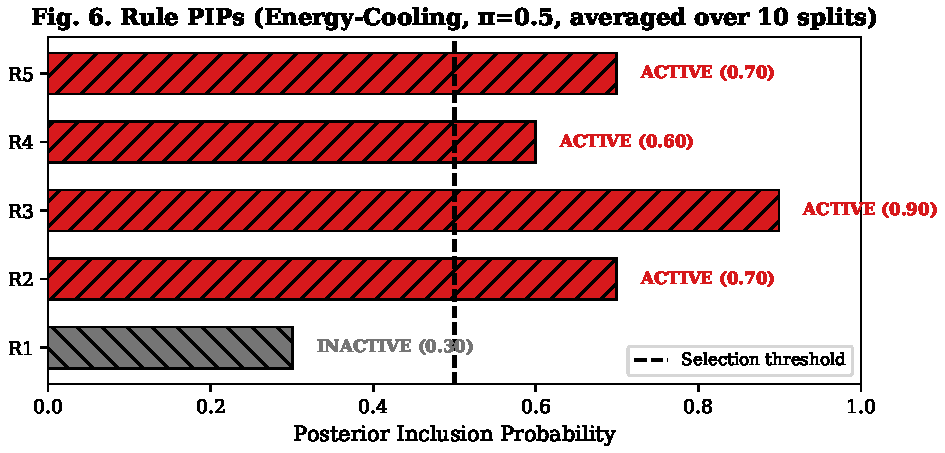
\includegraphics[width=0.85\columnwidth]{results/figures/fig6_rules.pdf}
\caption{Rule posterior inclusion probabilities (Energy-Cooling, $\pi=0.5$, averaged over 10 ablation splits). R2, R3, R5 are active (PIP $>0.5$); R1, R4 are pruned (38\% sparsity). Shaded bars indicate active rules; hatched bars indicate inactive rules.}
\label{fig:rules}
\end{figure}

%============================================================
\section{Discussion}
\label{sec:discussion}

\subsection{When Is Sparsity Worth the Accuracy Cost?}

The central tension in our results is between rule reduction and predictive performance. On the Energy datasets, pruning 38\% of rules incurs a 3.4--3.8$\times$ RMSE increase relative to dense TSK-LS (Table~\ref{tab:main}). Whether this trade-off is acceptable depends on the application context. In architectural design exploration, where engineers iterate through hundreds of building configurations, a 38\% reduction in rules to inspect may justify a moderate accuracy loss if the remaining rules preserve the correct qualitative relationships between building parameters and energy performance. However, for quantitative energy certification or compliance checking, the dense Bayesian-TSK baseline---which achieves both superior accuracy (RMSE $=3.57$--$4.11$) and calibrated intervals (PICP $=0.94$--$0.96$) on Energy data---is clearly the preferred choice. The practical value of the sparse model depends on whether the three retained rules correctly identify the most influential building parameters; verifying this requires domain-specific case studies that we leave to future work.

The sparsity-accuracy tension is most severe in the low-$R$, low-$d$ setting studied here. With only $R=5$ rules covering 8 input dimensions, each rule governs a large region of the input space. Removing two rules eliminates approximately 40\% of the coverage, and the remaining three rules cannot compensate for the lost local structure. At larger $R$ (e.g., $R=9$, where 5.4 rules are retained for 40\% sparsity), the per-rule coverage is finer-grained, suggesting that sparsity may become less costly as $R$ increases. This hypothesis is consistent with the cluster count sensitivity results (Fig.~\ref{fig:fcm})---$k=9$ achieves RMSE 20.51 with 40\% sparsity, comparable to the $k=5$ result (RMSE 20.55, 38\% sparsity) despite a larger absolute number of retained rules.

\subsection{Why Does the Analytical Approximation Undercover?}

The systematic undercoverage of TSK-SpikeSlab (PICP $=0.057$--$0.315$) has a specific mathematical origin. The Laplace predictive covariance (Eq.~\ref{eq:predvar}) approximates the posterior over $\boldsymbol{\beta}$ as Gaussian centered at the ridge estimate, with covariance given by the inverse Hessian of the log-posterior. When rule $j$ is pruned (PIP $\leq 0.5$), the corresponding prior precision is set to $10^{10}$ (essentially zero variance), collapsing the marginal variance for all predictions that depend on that rule's parameters. However, the actual posterior over $\gamma_j$ is not concentrated at zero for pruned rules---the average PIP for R1 is 0.30 (Fig.~\ref{fig:rules}), meaning there remains a 30\% posterior probability that R1 should be included. The Laplace approximation ignores this model uncertainty entirely by conditioning on a single hard threshold.

The $\tau^2$ sensitivity results confirm this diagnosis: even at $\tau^2=10^6$, where the unpruned rules have an extremely diffuse prior, PICP only reaches 0.228 (Supplementary Table~S2). The undercoverage is not primarily caused by an overly narrow slab prior, but by the decision to discard rules rather than average over them. Full Bayesian model averaging---where predictions are weighted by each model's posterior probability---would produce wider intervals that reflect uncertainty about which rules are active. This is exactly the direction that MCMC or variational inference would enable.

\subsection{Implications for Sparse TSK System Design}

Our findings carry implications beyond the specific spike-and-slab implementation studied here. First, any sparse TSK method that selects rules via hard thresholding---whether through PIP, L$_1$ regularization path, or information criterion minimization---will face the same structural challenge: the weighted design matrix $\boldsymbol{\Phi}$ is inherently multicollinear (condition number $>10^{16}$ in our experiments), making the selection decision sensitive to small perturbations in the data. The LassoCV diagnostic (Section~\ref{sec:results}) demonstrates that L$_1$ regularization paths are particularly vulnerable: the standard $\alpha$ grid collapses predictions to near zero, while expanding the grid to $\alpha \to 0$ recovers the OLS solution---neither extreme is satisfactory.

Second, the choice of $\alpha$ in the ridge initialization step (Table~\ref{tab:ablation}) is the single most consequential hyperparameter for the analytical approximation, changing RMSE by 26.2 across the tested range. This sensitivity is not a weakness of our specific implementation but a consequence of the approximation strategy: the initial ridge fit propagates into every BIC computation, and errors in the initial $\boldsymbol{\beta}$ estimate cascade through all subsequent steps. Methods that avoid this two-stage structure---such as full MCMC, where $\boldsymbol{\beta}$ and $\boldsymbol{\gamma}$ are updated jointly---would not exhibit the same $\alpha$-sensitivity.

Third, the $\pi$ insensitivity result (RMSE varying by $<10^{-3}$ across $\pi\in[0.1,0.9]$) has a constructive interpretation: it confirms that the data dominate the prior in BIC-based selection when the Bayes factor is sufficiently large. For practitioners, this means that the choice of $\pi$ need not be a barrier to adoption---the method will produce consistent rule selections regardless of the prior inclusion probability. However, it also means that $\pi$ cannot be used to encode domain knowledge about expected sparsity levels, limiting the method's utility in applications where prior information about rule relevance is available.

\subsection{Comparison with Related Approaches}

Our work differs from Den{\oe}ux's ENNreg framework \cite{denoeux2023ennreg} in two fundamental respects. ENNreg models prediction uncertainty through random fuzzy sets and belief functions, producing a Dempster-Shafer belief distribution over output values. While ENNreg also generates prediction intervals for fuzzy regression, it does not perform rule-level variable selection---all rules contribute to every prediction, weighted by their belief masses. The spike-and-slab prior, by contrast, makes an explicit binary decision about each rule's inclusion, trading the continuity of ENNreg's belief-based weighting for the interpretability of hard rule removal. Which approach is preferable depends on whether the application prioritizes calibrated uncertainty (ENNreg) or compact rule bases (spike-and-slab).

Compared to continuous shrinkage priors such as the Horseshoe \cite{carvalho2010horseshoe}, the spike-and-slab prior offers a conceptual advantage for fuzzy rule selection: the binary inclusion indicator $\gamma_j$ directly maps to the engineer's decision of whether to inspect rule $j$, and the posterior inclusion probability provides an interpretable measure of evidence. The Horseshoe prior would shrink rule parameters toward zero without ever setting them exactly to zero, requiring an additional thresholding step that reintroduces the same hard-decision problem. However, the Horseshoe's continuous shrinkage may achieve a smoother bias-variance trade-off in practice, making it a natural candidate for future comparisons.

\subsection{Limitations and Future Directions}

Beyond the three limitations discussed in Section~\ref{sec:conclusion}, several additional constraints merit attention. The current study uses only two UCI benchmark datasets with $d=8$---a dimensionality regime where sparsity is a convenience rather than a necessity. We expect the relative advantage of spike-and-slab selection to grow with dimensionality; in $d>30$ settings, dense TSK models accumulate $R(d+1)>150$ parameters, and the overfitting risk that motivates this work becomes acute. The building energy domain provides a natural pathway to higher dimensions: real building energy models often include 20--50 design parameters (orientation, glazing ratios, HVAC specifications, occupancy schedules), and simulation-based datasets with $n \approx 500$--$2000$ are common in practice.

A second direction concerns the antecedent structure. Our method treats antecedents as fixed (derived from $k$-means clustering) and applies sparsity only to consequents. Joint antecedent-consequent selection---where rules with uninformative consequents also trigger revision of the corresponding fuzzy partition---would provide a more complete sparse TSK framework. Recent work on joint structure identification in Bayesian TSK \cite{gu2018bayesian} provides a natural starting point, though extending it to incorporate spike-and-slab priors introduces computational challenges.

Finally, the practical deployment of sparse TSK systems in building energy applications requires validation against measured (rather than simulated) energy consumption data. The Energy Efficiency dataset used here is generated by Ecotect simulation software under idealized conditions; real buildings exhibit occupant-driven variability, sensor noise, and temporal dynamics that may alter the sparsity patterns observed. A field study pairing sparse TSK models with submetered building energy data would strengthen the application-driven case that ASC prioritizes.

%============================================================
\section{Conclusion}
\label{sec:conclusion}

We introduced spike-and-slab priors for TSK fuzzy rule consequent selection, with an analytical BIC-based approximation that performs rule selection and parameter estimation without MCMC sampling. Empirical evaluation on three benchmarks reveals a data-dependent sparsity pattern: 38\% rule reduction on the Energy datasets (1.9 of 5 rules pruned) but no pruning on Concrete (5.0 of 5 retained). The non-sparse conjugate Bayesian TSK baseline achieves well-calibrated prediction intervals (PICP $=0.900$--$0.961$), confirming that the conjugate Gaussian--Wishart framework provides reliable uncertainty estimates for dense TSK systems. However, the spike-and-slab variant---which uses a Laplace covariance approximation---systematically undercovers after rule pruning (PICP $=0.057$--$0.315$), revealing that analytical approximations cannot simultaneously deliver sparsity, competitive accuracy, and calibrated uncertainty at the data scales studied here. Mechanism analysis confirms that Bayesian predictive uncertainty distinguishes regions where the spike-and-slab prior outperforms uniform L$_1$ shrinkage.

Three limitations define the scope of these findings and motivate future work. First, the BIC-based approximation implements spike-and-slab selection as hard thresholding at PIP $>0.5$, which discards rules entirely and incurs a severe accuracy penalty in low-dimensional settings ($d=8$, $R=5$). Continuous shrinkage priors (e.g., the Horseshoe) or full MCMC implementations \cite{george1993variable} may achieve a smoother sparsity-accuracy trade-off by retaining partial information from near-zero rules. Second, the Laplace predictive approximation collapses after rule pruning; replacing it with variational inference or bootstrap-based intervals would directly address the undercoverage observed here. Third, the low-dimensional UCI benchmarks ($d=8$) limit the observable benefit of sparsity; we expect compounding advantages in $d>30$ settings, where dense TSK models have $R(d+1) > 150$ parameters and sparsity is essential rather than optional. Closing the gap between analytical approximations and full Bayesian inference for sparse TSK systems remains an open challenge with clear practical motivation.

\section*{Acknowledgments}

The author declares no specific funding for this research.

\section*{Data Availability}

Datasets are publicly available from the UCI Machine Learning Repository: Energy Efficiency (dataset 242) \cite{tsanas2012accurate} and Concrete Compressive Strength (dataset 165) \cite{yeh1998modeling}. Code is available at \texttt{https://github.com/Jackxiaozhiren/tsk-spikeslab}.

\section*{Conflict of Interest}

The authors declare no competing interests.

\bibliographystyle{elsarticle-num}
\bibliography{references}

\end{document}
